\documentclass[12pt]{amsart}
\usepackage{enumerate}
\usepackage[colorlinks=true, linkcolor=blue, urlcolor=blue, citecolor=blue, anchorcolor=blue, pdfborder={0 0 0}]{hyperref}
\usepackage{url}
\usepackage{graphicx,color}
\usepackage{cite}
\usepackage{amsthm, amsmath, amssymb}
\usepackage{mathtools}
\usepackage[top=45truemm, bottom=45truemm, left=30truemm, right=30truemm]{geometry}
\usepackage{nicefrac}
\usepackage{cancel}
\usepackage{float}
\usepackage{tabularx}
\usepackage{makecell}
\usepackage{array}
\usepackage{ragged2e}

\newcolumntype{P}[1]{>{\RaggedRight\hspace{0pt}}p{#1}}
\newcolumntype{L}{>{\begin{math}}l<{\end{math}}}%
\newcolumntype{C}{>{\begin{math}}c<{\end{math}}}%
\newcolumntype{R}{>{\begin{math}}r<{\end{math}}}%

\newtheorem{theorem}{Theorem}[section]
\newtheorem{lemma}[theorem]{Lemma}
\newtheorem{corollary}[theorem]{Corollary}
\newtheorem{definition}[theorem]{Definition}
\newtheorem{proposition}[theorem]{Proposition}
\newtheorem{example}[theorem]{Example}
\theoremstyle{definition}
\newtheorem{remark}[theorem]{Remark}

\setlength{\headsep}{2em}
\setlength{\skip\footins}{1.4pc plus 5pt minus 2pt}

\title[Engel Expansions in Collatz Sequences]{The Role of Engel Expansions in Collatz Sequences}

\author[F.\ Last1]{\href{https://orcid.org/0000-0000-0000-0000}{
\includegraphics[scale=0.06]{orcid.png}}\hspace{1mm}First Last}
\address{First Lastname\\
Graduate School of Mathematics\\ XYZ University\\ City\\ Adresszusatz\\ ZIP\\ Germany}
\curraddr{}
\email{first.last@university.de}

\author[F.\ Last2]{First Last}
\address{First Lastname\\
Graduate School of Mathematics\\ XYZ University\\ City\\ Adresszusatz\\ ZIP\\ Germany}
\curraddr{}
\email{first.last@university.de}

\subjclass[2010]{37P99}
\keywords{Engel Expansions, Collatz Sequences}

\begin{document}
	
\begingroup
\let\MakeUppercase\relax
\maketitle
\endgroup

\begin{abstract}
The Collatz conjecture is a number theoretical problem, which has puzzled countless researchers using myriad approaches. Presently, there are scarcely investigations to treat the problem from the angle of the question "which are the corner cases the Collatz Sequences?". We pursue this question and to this end examine ascending continued fractions -- the so called Engel expansions. We demonstrate that Engel expansions form worst case sequences $v_1,v_2,\ldots,v_n,v_{n+1}$ maximizing $v_{n+1}$ and maximizing the product $(1+\nicefrac{1}{3v_1})(1+\nicefrac{1}{3v_2})\cdots(1+\nicefrac{1}{3v_n})(1+\nicefrac{1}{3v_{n+1}})$.
\end{abstract}

\section{Introduction}
\label{introduction}
The Collatz conjecture is a well-known number theory problem and is the subject of numerous publications. An overview is provided by Lagarias \cite{Ref_Lagarias_2010}. Therefore, our description of the topic will be brief. The mathematician Lothar Collatz introduced a function $g:\mathbb{N}\rightarrow\mathbb{N}$ as follows:

\begin{equation}
\label{eq:func_collatz}
g(x)=
\begin{cases}
3x+1	&	2\nmid x\\
x/2		&	\text{otherwise}
\end{cases}
\end{equation}

\par\medskip
In the following, we only consider compressed Collatz sequences that solely contain the odd members, such as described by Bruckman \cite{Ref_Bruckman_2008}, who used the more convenient function that opts out all even integers:

\begin{equation}
\label{eq:func_collatz_odd}
f(x)=(3x+1)\cdot2^{-\alpha(x)},\text{where}\hspace{1em}2^{\alpha(x)}\mathrel\Vert(3x+1)
\end{equation}

\par\medskip
Note that $\alpha(x)$ is the largest possible exponent for which $2^{\alpha(x)}$ exactly divides $3x+1$. Especially for prime powers, one often says $p^\alpha$ \textit{divides} the integer $x$ \textit{exactly}, denoted as $p^\alpha\mathrel\Vert x$, if $p^\alpha$ is the greatest power of the prime $p$ that divides $x$.

\newpage
\begin{definition}
\label{def:halting_conditions}
A (compressed) Collatz sequence $v_1,v_2,\ldots,v_n,v_{n+1}$ ends when one of the following two conditions is reached:

\[
\begin{array}{ll}
\text{1.}&v_{n+1}=1\\[\medskipamount]
\text{2.}&v_{n+1}\in\{v_1,v_2,v_3,\ldots,v_n\}
\end{array}
\]

When the first condition applies, the Collatz conjecture is true for a specific sequence. If the second condition is fulfilled, the sequence has led to a cycle.
\end{definition}

\par\bigskip\noindent
A Collatz sequence $v_1,v_2,\ldots,v_n,v_{n+1}$ allowed at most one division by $2$ between two successive members. Dividing only once between two successive members, maximizes $v_{n+1}$. Such a sequence forms the following ascending continued fraction (cf. also \cite[p.~11]{Ref_Laarhoven}):
\begin{equation}
\label{eq:engel_k3}
v_{n+1}=\cfrac{3\cfrac{3\cfrac{3\cfrac{3v_1+1}{2}+1}{2}+1}{2}+1}{2}\dotsb
=\frac{3^nv_1+\sum_{i=0}^{n-1}3^i2^{n-1-i}}{2^n}
=\frac{3^n(v_1+1)-2^n}{2^n}
\end{equation}

\medskip
\begin{example}
\label{ex:engel_31}
A concrete example for such a sequence is $v_1=31$, $v_2=47$, $v_3=71$, $v_4=107$, $v_5=161$. And, to follow that example, we can calculate $v_5$ in a straightforward way:
\[
v_5=v_{n+1}=\frac{3^4(31+1)-2^4}{2^4}=161
\]

\par\medskip
Besides, by choosing a starting number $v_1=2^{n+1}-1$, we are able to infinitely generate sequences each forming an ascending continued fraction. As per equation~\ref{eq:engel_k3} the last member in this sequence is the odd number $v_{n+1}=3^n\cdot2-1$.
\end{example}

\medskip
\begin{remark}
Ascending variants of a continued fraction, such as used in equation~\ref{eq:engel_k3}, shall not be confused with continued fractions as treated in \cite{Ref_Moore}, \cite{Ref_Hensley}, \cite{Ref_Borwe_etal}. Ascending continued fractions used in our case correspond to the so-called "Engel Expansions" \cite{Ref_Kraaikamp_Wu}.
\end{remark}

\par\noindent
As illustrated below, we can formulate the ascending continued fractions in a generalized fashion, whereas the analogy to \ref{eq:engel_k3} is given by $b_1=b_2=b_3=b_4=2$ and $a_1=3^0$, $a_2=3^1$, $a_3=3^2$ and $a_4=3^3+3^4v_1$:

\[
\cfrac{a_1+\cfrac{a_2+\cfrac{a_3+\cfrac{a_4}{b_4}}{b_3}}{b_2}}{b_1}\dotsb=\frac{a_1}{b_1}+\frac{a_2}{b_1b_2}+\frac{a_3}{b_1b_2b_3}+\frac{a_4}{b_1b_2b_3b_4}+\cdots
\]

\par\medskip
The generalized form of equation~\ref{eq:engel_k3} may be used to compute any of the above-named ascending continued fraction that has $a_i=k^{i-1}$, $b_i=b$ for $i\in\mathbb{N}$ and $a_n=k^{n-1}+k^nv_1$:

\begin{equation}
\label{eq:generalized_asc_continued_fraction}
v_{n+1}=\frac{k^n(kv_1-bv_1+1)-b^n}{b^n(k-b)}
\end{equation}

\par\medskip\noindent
Table~\ref{table:engel_expansions_k_1_3_5_7} provides for $k=1,3,5,7$ each formula that calculates $v_{n+1}$ of an Engel expansion along with some example sequences. We obtained these formulas by inserting $b=2$ and $k=1,3,5,7$ into equation~\ref{eq:generalized_asc_continued_fraction}.

{\renewcommand{\arraystretch}{1.8}
\begin{table}[H]
	\centering
	\begin{tabular}{|L|L|L|L|}
		\hline
		\thead{\boldsymbol{k}} &
		\thead{\textbf{equation for~}\boldsymbol{v_{n+1}}} &
		\thead{\textbf{example sequence}} &
		\thead{\textbf{resulting}~\boldsymbol{v_{n+1}}}\\
		\hline
		1
		& v_{n+1}=\frac{v_1-1+2^n}{2^n}
		& 513,257,129,65,33,17,9,5,3
		& v_9=\frac{513-1+2^8}{2^8}=3
		\\ \hline
		3
		& v_{n+1}=\frac{3^n(v_1+1)-2^n}{2^n}
		& 127,191,287,431,647,971,1457
		& v_7=\frac{3^6(127+1)-2^6}{2^6}=1457
		\\ \hline
		5
		& v_{n+1}=\frac{5^n(3v_1+1)-2^n}{3\cdot2^n}
		& 85,213,533,1333,3333,8333
		& v_6=\frac{5^5(3\cdot85+1)-2^5}{3\cdot2^5}=8333
		\\ \hline
		7
		& v_{n+1}=\frac{7^n(5v_1+1)-2^n}{5\cdot2^n}
		& 51,179,627,2195,7683
		& v_5=\frac{7^4(5\cdot51+1)-2^4}{5\cdot2^4}=7683
		\\ \hline
	\end{tabular}
	\caption{Some exemplary Engel expansions for $b=2$ and $k=1,3,5,7$}
	\label{table:engel_expansions_k_1_3_5_7}
\end{table}}

\section{Include more divisions by two into an Engel expansion}
\label{sec:include_divisions_engel_expansion}
For calculating the largest possible $v_{n+1}$, we considered so far Engel expansions which contain only $n$ division by two within a Collatz sequence of $n+1$ memebers. In the following we include $m$ additional divisions by two and thus a total of $m+n$ divisions.

\par\medskip
Our starting point again is a Collatz sequence $v_1,v_2,\ldots,v_{n+1}$ consisting of $n+1$ members. We have a total of $m+n$ divisions by two that are distributed over $n$ positions:

\begin{equation}
\label{eq:alpha_n_m}
\alpha=n+m=\alpha_1+\alpha_2+\cdots+\alpha_n
\end{equation}

The number of positive integer solutions of the diophantine equation above is given by the following binomial coefficient, which is commonly used to calculate combinations with repetition, see \cite[p.~54]{Ref_Brualdi_2010}:

\[
\binom{n+(\alpha-n)-1}{\alpha-n}=\binom{n+m-1}{m}
\]

\par\medskip
Each of these solutions describes a possible way to distribute the $m+n$ divisions by two across $n$ positions within a Collatz sequence containing $n+1$ members. But how do we distribute these divisions in such a way that $v_{n+1}$ becomes maximum? This is precisely the case if as many divisions as possible are performed right at the beginning, which is illustrated in appendix~\ref{appx:permuting_divisions}. The Engel expansion of this case (that maximizes the value of $v_{n+1}$) provides the following formula for calculating the last sequence member $v_{n+1}$:

\begin{equation}
\label{eq:engel_more_divisions}
v_{n+1}=\left(\frac{k}{2}\right)^{n-1}\left(\frac{kv_1+1}{2^{\alpha_1}}+\frac{1}{k-2}\right)-\frac{1}{k-2}=\left(\frac{k}{2}\right)^{n-1}\left(v_2+\frac{1}{k-2}\right)-\frac{1}{k-2}
\end{equation}

\medskip
\begin{example}
	\label{ex:engel_67}
	We choose the sequence for $k=5$ starting at $v_1=67$ continuing with $v_2=21$, $v_3=53$, $v_4=133$, $v_5=333$, $v_6=833$ and $v_7=2083$. The last sequence member can be calculated by equation~\ref{eq:engel_more_divisions} directly as follows:
	
	\[
	v_7=\left(\frac{5}{2}\right)^{6-1}\left(21+\frac{1}{5-2}\right)-\frac{1}{5-2}=2083
	\]
\end{example}

\par\medskip\noindent
Moreover theorem~\ref{theo:permutation} specifies the limitation of the effect, which the division permutations have on the last sequence member $v_{n+1}$. As demonstrated in appendix~\ref{appx:permuting_divisions}, the maximum impact on $v_{n+1}$ of permuting division by two in a given Collatz sequence can be calculated by the difference between the highest and lowest possible value of $v_{n+1}$.

\par\medskip
\begin{theorem}
	\label{theo:permutation}
	Let $v_1,v_2,\ldots,v_n,v_{n+1}$ be a sequence in which a total of $n+m$ divisions by two took place. No matter how these divisions are permuted, i.e. performed sooner or later, the last member $v_{n+1}$ can differ at most by the following product:
	
	\[
	\left(\frac{3^{n-1}}{2^{n-1}}-1\right)\left(1-\frac{1}{2^m}\right)
	\]
\end{theorem}

\newpage
\section{Sum of reciprocated Collatz members}
\label{sum_reciprocal_vertices}
A product $\prod(1+a_n)$ with positive terms $a_n$ is convergent if the series $\sum a_n$ converges, see Knopp \cite[p.~220]{Ref_Knopp}. A similar statement provides Murphy \cite{Ref_Murphy}, who write the factors in the form $c_n=1+a_n$ and explains that if $\prod c_n$ is convergent then $c_n\rightarrow1$ and therefore if $\prod (1+a_n)$ is convergent then $a_n\rightarrow0$.

\par\medskip
We write the sum of reciprocated Collatz members as $\nicefrac{1}{kv_1}+\nicefrac{1}{kv_2}+\ldots+\nicefrac{1}{kv_n}+\nicefrac{1}{kv_{n+1}}$. In order to formulate this sum independently from the successive members $v_2,v_3,\ldots$, we substitute these as follows:

\begin{flalign}
v_1&=v_1\notag\\
v_2&=\frac{kv_1+1}{2^{\alpha_1}}\notag\\
v_3&=\frac{k^2v_1+k+2^{\alpha_1}}{2^{\alpha_1+\alpha_2}}\notag\\
v_4&=\frac{k^3v_1+k^2+k\cdot2^{\alpha_1}+2^{\alpha_1+\alpha_2}}{2^{\alpha_1+\alpha_2+\alpha_3}}\label{eq:sum_v_4}\\
\vdots\notag\\
v_{n+1}&=\frac{k^nv_1+\sum_{j=1}^{n}k^{j-1}2^{\alpha_1+\ldots+\alpha_n-\sum_{l>n-j}\alpha_l}}{2^{\alpha_1+\ldots+\alpha_n}}\label{eq:sum_v_n_plus_1}
\end{flalign}

\par\medskip
The sum of the reciprocal Collatz sequence members can be expressed as a term that only depends from $v_1$ and from the number of dvisions by two $\alpha_1,\alpha_2,\alpha_3,\ldots$ between two successive members:
\begin{equation*}
\sum_{i=1}^{n+1}\frac{1}{kv_i}=\frac{1}{k}\left(\frac{1}{v_1}+\sum_{i=1}^{n}\frac{1}{v_{i+1}}\right)=\frac{1}{k}\left(\frac{1}{v_1}+\sum_{i=1}^{n}\frac{2^{\alpha_1+\ldots+\alpha_i}}{k^iv_1+\sum_{j=1}^{i}k^{j-1}2^{\alpha_1+\ldots+\alpha_n-\sum_{l>i-j}\alpha_l}}\right)
\end{equation*}

%\vspace{1em}
\section{The product of reciprocated Collatz members incremented by one}
\label{appx:product_formula_depending_v1}
In a similar way to deduce the sum of reciprocal vertices depending only on $v_1$ as performed in \ref{sum_reciprocal_vertices}, we evolve the formula for the product of reciprocated Collatz members (incremented by one):

\begin{flalign}
\prod_{i=1}^{n+1}\left(1+\frac{1}{kv_i}\right)&=1+\frac{2^{\alpha_1+\ldots+\alpha_n}+k\cdot2^{\alpha_1+\ldots+\alpha_{n-1}}+\ldots+k^{n-1}\cdot2^{\alpha_1}+k^n}{k^{n+1}v_1}\label{eq:prod_sum_v_n_plus_1}\\
&=1+\frac{2^{\alpha_1+\ldots+\alpha_n}+k\cdot\sum_{j=1}^{i}k^{j-1}2^{\alpha_1+\ldots+\alpha_n-\sum_{l>i-j}\alpha_l}}{k^{n+1}v_1}\label{eq:prod_sum_v_n_plus_1_inserted}\\
&=\frac{2^{\alpha_1+\ldots+\alpha_n}\left(1+kv_{n+1}\right)}{k^{n+1}v_1}\label{eq:prod_sum_v_n_plus_1_simplified}
\end{flalign}

We inserted the sum used in equation~\ref{eq:sum_v_n_plus_1} into the above-given equation~\ref{eq:prod_sum_v_n_plus_1} and then obtained equation~\ref{eq:prod_sum_v_n_plus_1_inserted}. Now let us divide this product by the last factor in order to retrieve the product which iterates to $n$ instead of $n+1$:

\begin{equation}
\label{eq:prod_sum_v_n_simplified}
\prod_{i=1}^{n}\left(1+\frac{1}{kv_i}\right)=\frac{\prod_{i=1}^{n+1}\left(1+\frac{1}{kv_i}\right)}{\frac{kv_{n+1}+1}{kv_{n+1}}}=\frac{2^{\alpha_1+\ldots+\alpha_n}v_{n+1}}{k^nv_1}
\end{equation}

\par\medskip
The above-shown equation~\ref{eq:prod_sum_v_n_simplified} becomes simplified, when we replaced the numerator by equation~\ref{eq:prod_sum_v_n_plus_1_simplified}. The question which sequence maximizes its last member $v_{n+1}$ ties into the question: Which sequence maximizes the product? The product formula~\ref{eq:prod_sum_v_n_simplified} does not depend from all vertices $v_1,v_2,\ldots,v_n$, it depends only from $2^\alpha=2^{\alpha_1+\ldots+\alpha_n}$, from the first sequence member $v_1$ and the final one $v_{n+1}$.

\section{Maximizing the product of reciprocated Collatz members}
Consider a Collatz sequence containing $n$ elements and starting at a given integer $v_1$. The corresponding product given by equation~\ref{eq:prod_sum_v_n_simplified} becomes largest if we
\begin{itemize}
\item maximize the last member $v_{n+1}$,
\item choose a smallest possible $v_1$ and
\item choose an $\alpha=n+m$ as large as possible, where $m$ is the crucial lever.
\end{itemize}

It is therefore a maximization problem over several variables. In the following we will reflect on how to approach a solution to the problem.

\par\medskip\noindent
{\bfseries\boldmath Minimizing $v_1$:} This is obvious and tricially achievable by iterating $v_1$ through small integers, starting at $v_1=1$.

\par\medskip\noindent
{\bfseries\boldmath Maximizing $\alpha$:} We must choose a Collatz sequence, in which as many divisions by two as possible occurred. Since $n$ and $m$ depend directly on $\alpha$, maximizing $\alpha$ is equivalent to maximizing $n$ or $m$. In general, adding more factors $(1+\nicefrac{1}{kv_i})$ can only increase the product. So, the larger $n$, the larger the product. Note that despite everything, $m$ is the key maximizer of the product -- these additional divisions by two reduce the sequence members $v_i$.

\par\medskip\noindent
{\bfseries\boldmath Maximizing $v_{n+1}$:} If we fix $v_1,\alpha,n$ then this maximum occurs when the sequence is an Engel expansion, id est when we run the most divisions by two at the beginning. Consequently, the exponent alpha (the total number of divisions by two) is the sum of a large $\alpha_1$ and the remaining alpha values which are all one:
\[
\alpha=n+m=\alpha_1+\alpha_2+\cdots+\alpha_n=\alpha_1+1+\cdots+1=\alpha_1+n-1
\]

The product of reciprocated Collatz members (incremented by one) for such an Engel expansion is given by the following equation:

\begin{flalign}
\label{eq:prod_engel_more_divisions}
\prod_{i=1}^{n}\left(1+\frac{1}{kv_i}\right)&=1+\frac{1}{kv_1}+\frac{2^{\alpha_1}}{k(k-2)v_1}\left(1-\left(\frac{2}{k}\right)^{n-1}\right)\\
\label{eq:prod_engel_more_divisions_v2}
&=1+\frac{1}{kv_1}+\frac{kv_1+1}{k(k-2)v_1v_2}\left(1-\left(\frac{2}{k}\right)^{n-1}\right)
\end{flalign}

\medskip
\begin{example}
	An example for $k=3$ provides the sequence $v_1=661$, $v_2=31$, $v_3=47$, and $v_4=71$. In this case $\alpha_1=6=m+1$ and $\alpha_2=\alpha_3=\alpha_4=1$. We now calcultae the product of reciprocated Collatz sequence members by inserting $v_1=661$ and $v_2=31$ together with $k=3$ and $n=4$ into equation~\ref{eq:prod_engel_more_divisions_v2}:
	
	\begin{flalign*}
	\prod_{i=1}^{4}\left(1+\frac{1}{3v_i}\right)&=
	\left(1+\frac{1}{3\cdot661}\right)\left(1+\frac{1}{3\cdot31}\right)\left(1+\frac{1}{3\cdot47}\right)\left(1+\frac{1}{3\cdot71}\right)\\
	&=1+\frac{1}{3\cdot 661}+\frac{3\cdot 661+1}{3\cdot(3-2)\cdot 661\cdot 31}\left(1-\left(\frac{2}{3}\right)^{4-1}\right)\\
	&=1.0232158532713247
	\end{flalign*}
\end{example}

\par\medskip
Maximizing the product of reciprocated Collatz sequence members $\prod_{i=1}^{n}(1+\nicefrac{1}{kv_i})$ requires us to maximize the equation~\ref{eq:prod_engel_more_divisions} or \ref{eq:prod_engel_more_divisions_v2}. This maximization is archieved by choosing $v_1$ as small as possible (which we already know). Additionally we need to select a largest possible $\alpha_1=m+1$ or a lowest possible $v_2$ (which is clear as well). Lastly, this maximization also requires the choice of a value $n$ as large as possible. To find the largest product, we iterate the variables $v_1$ and $n$ independently through integers $1,2,\ldots$ and calculate the product for each combination of the variable assignment using equation~\ref{eq:prod_engel_more_divisions_v2}. Alternatively, one can maximize equation~\ref{eq:prod_engel_more_divisions} or \ref{eq:prod_engel_more_divisions_v2} analytically for the different $k$.

\par\medskip
Table~\ref{table:product_equations_k_3_5_7} provides for $k=1,3,5,7$ the formula for calculating the Engel expansion's product. This table furthermore indicates the maximum cases along with the corresponding results for each product. Recall that we are not allowed to choose an arbitrarily large $n$ if we set $v_1=1$ because of the halting conditions given by definition~\ref{def:halting_conditions}. The case $v_1=3,v_2=5,n=\infty$ for $k=3$ disregards the halting condition, the value $n$ runs towards infinity and thus much further than allowed -- nevertheless, the product value converges towards $\nicefrac{4}{3}$. Note that for $n=1$ it does not matter what value $v_2$ takes -- it has no effect on the resulting product value.

{\renewcommand{\arraystretch}{1.8}
	\begin{table}[H]
		\centering
		\begin{tabular}{|L|L|L|L|}
			\hline
			\thead{\boldsymbol{k}} &
			\thead{\textbf{product formula}} &
			\thead{\textbf{maximum case}} &
			\thead{\textbf{resulting product}}\\
			\hline
			1 & 1+\frac{1}{v_1} + \frac{v_1+1}{-v_1v_2}\left(1-2^{n-1}\right) & v_1=1,n=1
			& 2
			\\ \hline
			3 & 1+\frac{1}{3v_1} + \frac{3v_1+1}{3v_1v_2}\left(1-\left(\frac{2}{3}\right)^{n-1}\right) & \makecell[l]{v_1=1,n=1\\v_1=3,v_2=5,n=\infty}
			& \frac{4}{3}
			\\ \hline
			5 & 1+\frac{1}{5v_1} + \frac{5v_1+1}{15v_1v_2}\left(1-\left(\frac{2}{5}\right)^{n-1}\right) & v_1=1,v_2=3,n=2
			& \frac{32}{25}
			\\ \hline
			7 & 1+\frac{1}{7v_1} + \frac{7v_1+1}{35v_1v_2}\left(1-\left(\frac{2}{7}\right)^{n-1}\right) & v_1=1,n=1
			& \frac{8}{7}
			\\ \hline
		\end{tabular}
		\caption{Formulas that calculate the Engel expansion's product for $k=1,3,5,7$}
		\label{table:product_equations_k_3_5_7}
\end{table}}

\begin{figure}
	\begin{center}
		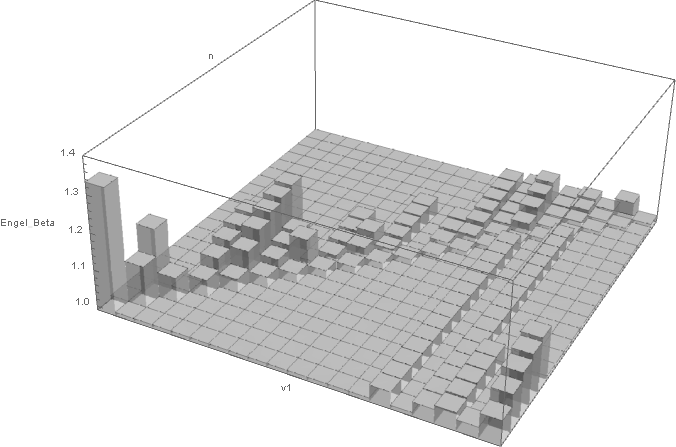
\includegraphics[width=1.0\textwidth]{plot.png}
		\caption{Chart that displays the Engel expansion's product value as a function of $v_1$ and $n$ for $k=3$}
		\label{fig:1}
	\end{center}
\end{figure}

\section{Pitfalls and limitations}
One may say that there exist some Collatz sequences, which are not an Engel expansions but their product might be larger than the product resulting from the corresponding Engel expansion. Let us take for example the following five-element sequence for $k=3$ starting at $v_1=7$ and finishing with $v_{n}=5$:
\[
\begin{array}{l@{\hspace{1em}}l@{\hspace{1em}}l@{\hspace{1em}}l@{\hspace{1em}}l@{\hspace{2em}}l}
v_1=7&v_2=11&v_3=17&v_4=13&v_5=5&v_{n+1}=v_6=1\\
\alpha_1=1&\alpha_2=1&\alpha_3=2&\alpha_4=3&\alpha_5=4&
\end{array}
\]

The total number of divisions by two within this sequence is $\alpha=11=n+m=5+6$. The product $(1+\nicefrac{1}{3v_1})\cdots(1+\nicefrac{1}{3v_5})$ of this sequence is $1.20399764$. If we insert into the Engel expansion product formula~\ref{eq:prod_engel_more_divisions_v2} analogously $v_1=7$ and $n=5$, it yields a product value of only $1.12404468$. Do not forget that in this case the value $\alpha=4$ is much lower. Let us shift the $m=6$ divisions to the beginning:
\[
\alpha=11=7+1+1+1+1=\alpha_1+1+1+1+1
\]
In this case we would obtain a (hypothetical) product value of $5.93885949$, which is quite larger. One may verify this by inserting $k=3,v_1=7,\alpha_1=7,n=5$ into equation~\ref{eq:prod_engel_more_divisions}. In the end, it is not sufficient to maximize only $v_{n+1}$, we need to optimize all parameters -- choose smallest possible $v1,v_2$ and largest number of $n$.

\par\medskip
One question that still is open is: Does there exist a sequence which is not an Engel expansion, but nevertheless has a greater product value by compensating a smaller $v_{n+1}$ through including more additional divisions by two (which means a larger $m$)?

%{\setlength{\jot}{1.2em}
%\begin{flalign}
%\label{eq:engel_k3_m}
%v_{n+1}&=\cfrac{3\cfrac{3\cfrac{3\cfrac{3v_1+1}{2\cdot2^m}+1}{2}+1}{2}+1}{2}\dotsb
%=\cfrac{3\cfrac{3\cfrac{3v_2+1}{2}+1}{2}+1}{2}\dotsb
%=\frac{3^{n-1}(v_2+1)-2^{n-1}}{2^{n-1}}\\
%\notag
%&=\frac{3^{n-1}(\frac{3v_1+1}{2\cdot2^{m}}+1)-2^{n-1}}{2^{n-1}}=\frac{3^nv_1+3^{n-1}+3^{n-1}2^{m+1}}{2^{m+n}}-1
%\end{flalign}}

\section{Condition for a limited growth of the Engel expansion}
\label{sec:condition_limited_growth}
Let us look now into the question of what condition must be met to prevent a greater growth than a decline in Collatz sequences. Specifically we consider an Engel expansion comprising $n+1$ sequence members that include $m$ additional divisions by two at the beginning. The last member $v_{n+1}$ in such a sequence can be calulated by formula~\ref{eq:engel_k3_m}. In order to restrict the growth of this sequence, we require that the last member has to be smaller than the first one. For this we define the condition $v_{n+1}<v_1$:

\[
\frac{3^nv_1+3^{n-1}+3^{n-1}2^{m+1}}{2^{m+n}}-1<v_1
\]

\par\medskip\noindent
Reshaping this inequality leads to the following condition:

\begin{equation}
\label{eq:condition_limited_growth}
\frac{3^{n-1}\left(2^{m+1}-2\right)}{2^{m+n}-3^n}-1<v_1
\end{equation}

\newpage
\section{Appendix}

\subsection{Permuting divisions by two}
\label{appx:permuting_divisions}
In order to illustrate how permuting divisions by two affect the last sequence member $v_{n+1}$, we take a look at two corner cases:
\begin{itemize}
	\item the one where we do the additional $m$ divisions by $2$ at the end and
	\item the one where we do these additional divisions at the very beginning.
\end{itemize}

\par\medskip\noindent
\textbf{The first case} is our starting point to examine how the swapping a division by two affects the sequence member $v_{n+1}$. For this, let us compare the Engel expansion where we devide by $2^m$ afterwards with one where we divide by $2$ in the penultimate step and by $2^{m-1}$ in last step. One can immediately recognize the following inequality with a mere look:
\[
\cfrac{1+\cfrac{3+\cfrac{3^2+\cfrac{3^3+3^4v_1}{2}}{2}}{2}}{2\cdot2^m}
<
\cfrac{1+\cfrac{3+\cfrac{3^2+\cfrac{3^3+3^4v_1}{2}}{2}}{2\cdot\textcolor{red}{\mathbf{2}}}}{2\cdot2^{m-1}}
\]

\par\bigskip
To put it simply, in the expansion on the right side of the above-shown inequality we perform one division by two a little bit earlier as we do it in the expansion on the left side of the expansion. Almost all summands of both expansions cancel out each other:

\[
\frac{1}{2\cdot2^m}+\cancel{\frac{3}{2^2\cdot2^m}+\frac{3^2}{2^3\cdot2^m}+\frac{3^3+3^4v_1}{2^4\cdot2^m}}
<
\frac{1}{2\cdot2^{m-1}}+\cancel{\frac{3}{2^2\cdot\textcolor{red}{\mathbf{2}}\cdot2^{m-1}}+\frac{3^2}{2^3\cdot\textcolor{red}{\mathbf{2}}\cdot2^{m-1}}\frac{3^3+3^4v_1}{2^4\cdot\textcolor{red}{\mathbf{2}}\cdot2^{m-1}}}
\]

\par\medskip\noindent
\textbf{The second case} deals with Engel expansions where we perform that additional $m$ divisions by two as early as possible. The resulting value $v_{n+1}$ decreases, when we make a division by two later:
\[
\cfrac{1+\cfrac{3+\cfrac{3^2+\cfrac{3^3+3^4v_1}{2\cdot2^{m-1}}}{2\cdot\textcolor{red}{\mathbf{2}}}}{2}}{2}
<
\cfrac{1+\cfrac{3+\cfrac{3^2+\cfrac{3^3+3^4v_1}{2\cdot2^m}}{2}}{2}}{2}
\]

\par\bigskip
Also here almost all summands of both Engel expansions, they cancel each other out:

\[
\cancel{\frac{1}{2}+\frac{3}{2^2}}+\frac{3^2}{2^3\cdot\textcolor{red}{\mathbf{2}}}+\cancel{\frac{3^3+3^4v_1}{2^4\cdot\textcolor{red}{\mathbf{2}}\cdot2^{m-1}}}
<
\cancel{\frac{1}{2}+\frac{3}{2^2}}+\frac{3^2}{2^3}+\cancel{\frac{3^3+3^4v_1}{2^4\cdot2^m}}
\]

\par\bigskip
While the first case minimizes the value of $v_{n+1}$, the second case maximizes it. The difference between the maximum and the minimum is given by the following equation:

\[
\frac{3^{n-1}\left(\frac{3v_1+1}{2\cdot2^m}+1\right)-2^{n-1}}{2^{n-1}}-\frac{3^n\left(v_1+1\right)-2^n}{2^{n+m}}=\left(\frac{3^{n-1}}{2^{n-1}}-1\right)\left(1-\frac{1}{2^m}\right)
\]
%\begin{flalign*}
%&\frac{3^{n-1}\left(\frac{3v_1+1}{2\cdot2^m}+1\right)-2^{n-1}}{2^{n-1}}-\frac{3^n\left(v_1+1\right)-2^n}{2^{n+m}}\\
%=&\frac{3^{n-1}\cdot\left(3v_1+1+2^{m+1}\right)-2^{n-1}\cdot2^{m+1}-3^n\left(v_1+1\right)+2^n}{2^{m+1}\cdot2^{n-1}}\\
%=&\frac{3^{n-1}+3^{n-1}\cdot2^{m+1}-2^{n+m}-3^n+2^n}{2^{n+m}}=\frac{3^{n-1}-3\cdot3^{n-1}+3^{n-1}\cdot2^{m+1}-2^{n+m}+2^n}{2^{n+m}}\\
%=&\frac{-2\cdot3^{n-1}+3^{n-1}\cdot2^{m+1}-2^{n+m}+2^n}{2^{n+m}}=\frac{\left(2\cdot3^{n-1}-2^n\right)\left(2^m-1\right)}{2^n\cdot2^m}\\
%=&\left(\frac{3^{n-1}}{2^{n-1}}-1\right)\left(1-\frac{1}{2^m}\right)
%\end{flalign*}

\par\bigskip
This has the consequence that for a given sequence consisting of $n+1$ members, between which a total of $n+m$ divisions have taken place, the permutations of these divisions have a limited effect on the last sequence member $v_{n+1}$ as described by theorem~\ref{theo:permutation}.

%\newpage
\vspace{1em}
\bibliographystyle{unsrt}
\bibliography{references}

\end{document}